\clearpage
\begin{trapbox}
\textbf{\textcolor{CTrap}{易错一：有镜像就一定有反函数}}
\begin{center}
\begin{minipage}{\linewidth}\centering
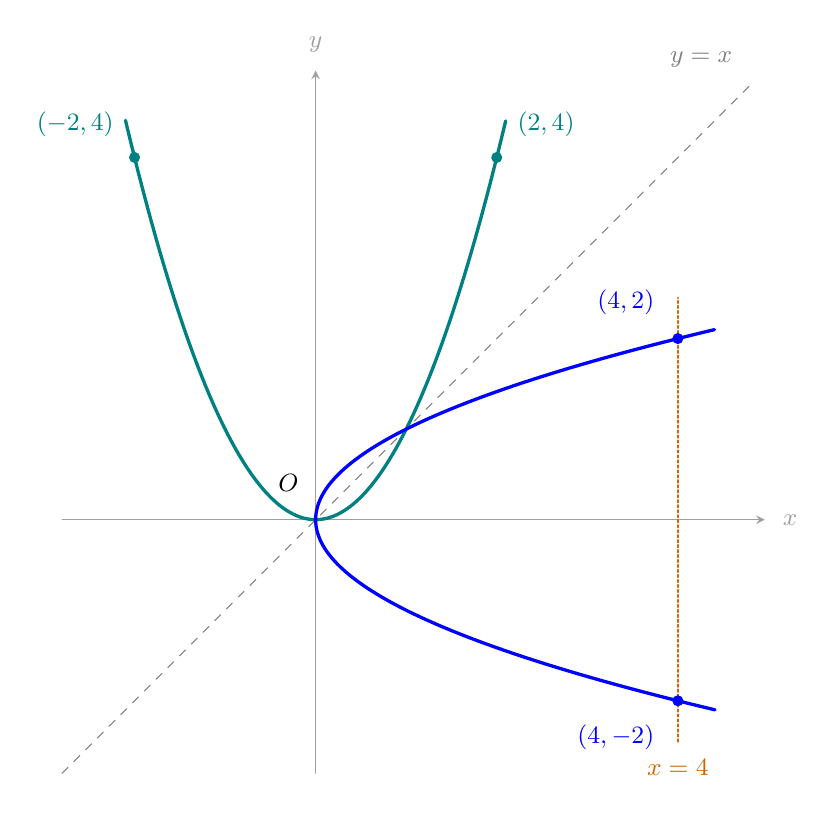
\begin{tikzpicture}[x=1.15cm,y=1.15cm,>=stealth,font=\small,line cap=round,line join=round]
\draw[->,gray!75] (-2.8,0)--(4.96,0) node[right=3pt]{$x$};
\draw[->,gray!75] (0,-2.8)--(0,4.96) node[above=3pt]{$y$};
\node at (-.3,.4) {$O$};
\draw[gray,dashed] (-2.8,-2.8)--(4.8,4.8) node[above left=3pt]{$y=x$};

\draw[teal,very thick,domain=-2.1:2.1,samples=121] plot(\x,{\x*\x});
\draw[blue,very thick,domain=-2.1:2.1,samples=121] plot({\x*\x},\x);
\draw[orange!80!black,densely dotted,thick] (4,-2.45)--(4,2.45);
\node[orange!80!black,below=3pt] at (4,-2.45) {$x=4$};
\fill[blue] (4,2) circle(2pt) node[above left=5pt]{$(4,2)$};
\fill[blue] (4,-2) circle(2pt) node[below left=5pt]{$(4,-2)$};
\fill[teal] (-2,4) circle(2pt) node[above left=4pt]{$(-2,4)$};
\fill[teal] (2,4) circle(2pt) node[above right=4pt]{$(2,4)$};

\end{tikzpicture}\par\smallskip
{\small \textcolor{teal}{\rule[.5ex]{1em}{.8pt}\ $y=x^2,\ x\in\mathbb R$}\qquad\textcolor{blue}{\rule[.5ex]{1em}{.8pt}\ $x=y^2$（镜像关系）}}\par
{\small 镜像在同一输入 $4$ 处有两个输出 $\pm2$，不能整体写成反函数。}\par\smallskip
\end{minipage}
\end{center}


$y=x^2$（$x\in\mathbb R$）的镜像是 $x=y^2$，在 $x=4$ 处有两个输出 $\pm2$，不构成一个普通函数。先限制到一一对应的分支，才可称反函数。
\end{trapbox}
\clearpage
\begin{trapbox}
\textbf{\textcolor{CTrap}{易错二：只交换式子，忘记交换范围}}
\begin{center}
\begin{minipage}{\linewidth}\centering
\begin{tikzpicture}[x=1.65cm,y=1.65cm,>=stealth,font=\small,line cap=round,line join=round]
\draw[->,gray!75] (-0.35,0)--(4.96,0) node[right=3pt]{$x$};
\draw[->,gray!75] (0,-0.35)--(0,4.96) node[above=3pt]{$y$};
\node at (-.3,.4) {$O$};
\draw[gray,dashed] (-0.15,-0.15)--(4.8,4.8) node[above left=3pt]{$y=x$};

\draw[teal,very thick,domain=0:1.5,samples=100] plot({1+\x},{2+\x*\x});
\draw[blue,very thick,domain=0:1.5,samples=100] plot({2+\x*\x},{1+\x});
\draw[orange!80!black,densely dotted] (1,2)--(2,1);
\fill[teal] (1,2) circle(2pt) node[left=6pt]{$(1,2)$};
\fill[blue] (2,1) circle(2pt) node[below=6pt]{$(2,1)$};

\end{tikzpicture}\par\smallskip
{\small \textcolor{teal}{\rule[.5ex]{1em}{.8pt}\ $y=(x-1)^2+2,\ x\ge1$}\qquad\textcolor{blue}{\rule[.5ex]{1em}{.8pt}\ $y=1+\sqrt{x-2},\ x\ge2$}}\par
{\small 原端点 $(1,2)$ 变为 $(2,1)$，范围限制随坐标一起交换。}\par\smallskip
\end{minipage}
\end{center}


$y=(x-1)^2+2,\ x\ge1$ 的镜像须带 $y\ge1$。不能选负根，也不能让反函数定义域取全体实数。正确反函数为 $1+\sqrt{x-2}$，定义域 $x\ge2$。
\end{trapbox}
\clearpage
\begin{trapbox}
\textbf{\textcolor{CTrap}{易错三：把反函数当作倒数}}
\begin{center}
\begin{minipage}{\linewidth}\centering
\begin{tikzpicture}[x=1.35cm,y=1.35cm,>=stealth,font=\small,line cap=round,line join=round]
\draw[->,gray!75] (-3.3,0)--(3.46,0) node[right=3pt]{$x$};
\draw[->,gray!75] (0,-3.3)--(0,3.46) node[above=3pt]{$y$};
\node at (-.3,.4) {$O$};
\draw[gray,dashed] (-3.3,-3.3)--(3.3,3.3) node[above left=3pt]{$y=x$};

\draw[teal,very thick,domain=-3:1.65,samples=121] plot(\x,{2^\x});
\draw[blue,very thick,domain=-3:1.65,samples=121] plot({2^\x},\x);
\draw[orange!80!black,very thick,dash dot,domain=-1.65:3,samples=121] plot(\x,{2^(-\x)});
\fill[blue] (2,1) circle(2pt) node[below right=5pt]{$(2,1)$};
\fill[orange!80!black] (2,.25) circle(2pt) node[below=15pt]{$(2,1/4)$};

\end{tikzpicture}\par\smallskip
{\small \textcolor{teal}{\rule[.5ex]{1em}{.8pt}\ $f(x)=2^x$}\qquad\textcolor{blue}{\rule[.5ex]{1em}{.8pt}\ $f^{-1}(x)=\log_2x$}\\[3pt]\textcolor{orange!80!black}{$1/f(x)=2^{-x}$（点划线）}}\par
{\small 镜像得到反函数；取函数值的倒数得到另一条曲线。}\par\smallskip
\end{minipage}
\end{center}


$f(x)=2^x$ 的反函数为 $\log_2 x$，而 $1/f(x)=2^{-x}$ 是另一个函数。反函数记号 $f^{-1}$ 表示输入输出互换，不是数值的倒数。
\end{trapbox}
\clearpage
\begin{trapbox}
\textbf{\textcolor{CTrap}{易错四：原函数和反函数的交点都在 $y=x$ 上}}
\begin{center}
\begin{minipage}{\linewidth}\centering
\begin{tikzpicture}[x=1.8cm,y=1.8cm,>=stealth,font=\small,line cap=round,line join=round]
\draw[->,gray!75] (-0.8,0)--(4.06,0) node[right=3pt]{$x$};
\draw[->,gray!75] (0,-0.8)--(0,4.06) node[above=3pt]{$y$};
\node at (-.3,.4) {$O$};
\draw[gray,dashed] (-0.15,-0.15)--(3.9,3.9) node[above left=3pt]{$y=x$};

\draw[teal,very thick] (-.4,3.4)--(3.4,-.4);
\fill[teal] (0,3) circle(2pt) node[left=6pt]{$(0,3)$};
\fill[teal] (3,0) circle(2pt) node[below left=8pt]{$(3,0)$};
\fill (1.5,1.5) circle(2pt) node[right=10pt]{$(3/2,3/2)$};

\end{tikzpicture}\par\smallskip
{\small \textcolor{teal}{$y=3-x$：原函数与反函数重合，整条直线都是公共点}}\par
{\small $(0,3)$ 与 $(3,0)$ 是公共点，却都不在对称轴上。}\par\smallskip
\end{minipage}
\end{center}


$f(x)=3-x$ 严格递减且 $f^{-1}=f$，全部直线点都是交点，例如 $(0,3)$。严格递增是保证可直接把交点问题化为 $f(x)=x$ 的充分条件；递减时需另外判断。
\end{trapbox}
\clearpage
\begin{trapbox}
\textbf{\textcolor{CTrap}{易错五：镜像斜率写成负倒数}}
\begin{center}
\begin{minipage}{\linewidth}\centering
\begin{tikzpicture}[x=1.35cm,y=1.35cm,>=stealth,font=\small,line cap=round,line join=round]
\draw[->,gray!75] (-3.3,0)--(3.46,0) node[right=3pt]{$x$};
\draw[->,gray!75] (0,-3.3)--(0,3.46) node[above=3pt]{$y$};
\node at (-.3,.4) {$O$};
\draw[gray,dashed] (-3.3,-3.3)--(3.3,3.3) node[above left=3pt]{$y=x$};

\draw[teal,very thick] (-1.5,-3)--(1.5,3);
\draw[blue,very thick] (-3,-1.5)--(3,1.5);
\draw[teal,densely dotted,thick] (0,0)--(1,0)--(1,2);
\draw[blue,densely dotted,thick] (0,0)--(0,1)--(2,1);
\node[teal,below=5pt] at (.5,0) {$1$};
\node[teal] at (1.4,1.9) {$2$};
\node[blue,left=5pt] at (-.2,.8) {$1$};
\node[blue] at (1.75,1.35) {$2$};
\fill[teal] (1,2) circle(2pt);
\fill[blue] (2,1) circle(2pt);

\end{tikzpicture}\par\smallskip
{\small \textcolor{teal}{\rule[.5ex]{1em}{.8pt}\ $y=2x,\ k=2/1=2$}\qquad\textcolor{blue}{\rule[.5ex]{1em}{.8pt}\ $y=x/2,\ k^\prime=1/2$}}\par
{\small 横纵增量互换，斜率互为倒数，符号保持不变。}\par\smallskip
\end{minipage}
\end{center}


原斜率 $2$ 的镜像斜率为 $1/2$，不是 $-1/2$。负倒数是两条非水平非竖直直线垂直时的关系。只有连接非重合镜像点的线段才与对称轴垂直。水平线与竖直线镜像互换。
\end{trapbox}
\clearpage
\begin{trapbox}
\textbf{\textcolor{CTrap}{易错六：忽略复合的定义域和全域条件}}
\begin{center}
\begin{minipage}{\linewidth}\centering
\begin{tikzpicture}[x=1.35cm,y=1.35cm,>=stealth,font=\small,line cap=round,line join=round]
\draw[->,gray!75] (-3.3,0)--(3.46,0) node[right=3pt]{$x$};
\draw[->,gray!75] (0,-3.3)--(0,3.46) node[above=3pt]{$y$};
\node at (-.3,.4) {$O$};
\draw[gray,dashed] (-3.3,-3.3)--(3.3,3.3) node[above left=3pt]{$y=x$};

\draw[teal,very thick,domain=-1.8:1.8,samples=121] plot(\x,{\x*\x});
\draw[orange!80!black,very thick,dash dot,domain=-1.35:1.35,samples=121] plot(\x,{(\x)^4});
\fill (1,1) circle(2pt) node[below right=7pt]{$(1,1)$};
\draw[gray,densely dotted] (1.3,1.3)--(1.3,{1.3^4});
\fill[orange!80!black] (1.3,{1.3^4}) circle(2pt);

\end{tikzpicture}\par\smallskip
{\small \textcolor{teal}{$f(x)=x^2$}\qquad\textcolor{gray}{$y=x$（灰虚线）}\\[3pt]\textcolor{orange!80!black}{$f(f(x))=x^4$（点划线）}}\par
{\small $x^4=x$ 在少数点成立，不代表 $f(f(x))=x$ 在全域成立。}\par\smallskip
\end{minipage}
\end{center}


要判定自身对称，需对每个 $x\in D$ 都有 $f(x)\in D$ 且 $f(f(x))=x$。例如 $f(x)=x^2$ 在 $\mathbb R$ 上虽然 $f(f(0))=0,f(f(1))=1$，但 $f(f(2))=16\ne2$；少数点验证不够。
\end{trapbox}
\clearpage
\begin{trapbox}
\textbf{\textcolor{CTrap}{易错七：反函数导数在同一个横坐标取倒数}}
\begin{center}
\begin{minipage}{\linewidth}\centering
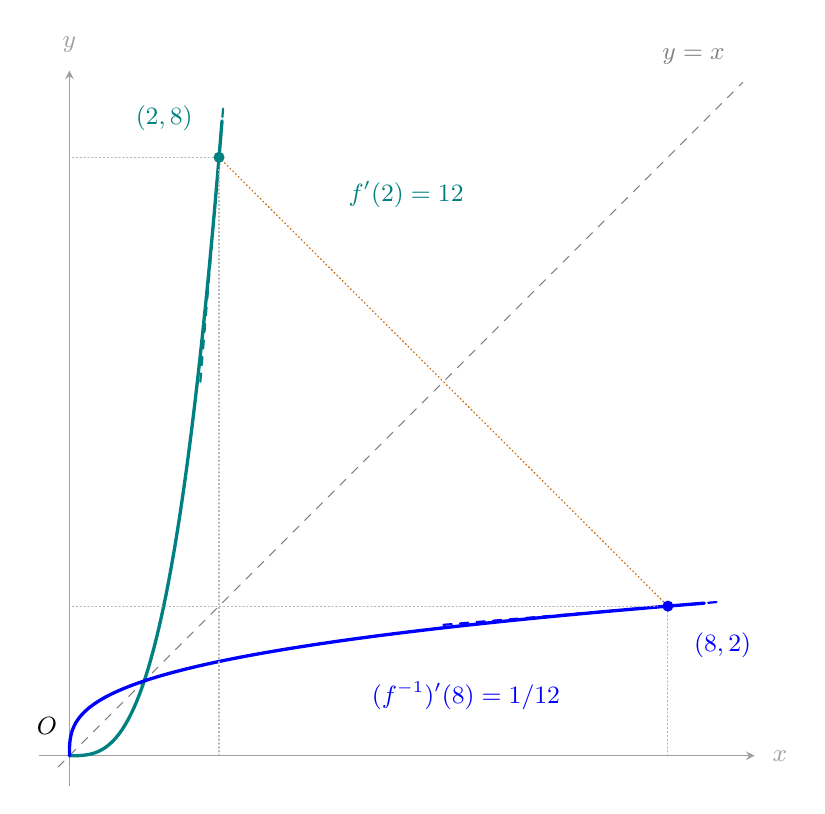
\begin{tikzpicture}[x=0.95cm,y=0.95cm,>=stealth,font=\small,line cap=round,line join=round]
\draw[->,gray!75] (-0.4,0)--(9.16,0) node[right=3pt]{$x$};
\draw[->,gray!75] (0,-0.4)--(0,9.16) node[above=3pt]{$y$};
\node at (-.3,.4) {$O$};
\draw[gray,dashed] (-0.15,-0.15)--(9,9) node[above left=3pt]{$y=x$};

\draw[teal,very thick,domain=0:2.04,samples=121] plot(\x,{\x^3});
\draw[blue,very thick,domain=0:2.04,samples=121] plot({\x^3},\x);
\draw[gray!60,densely dotted] (2,0)--(2,8)--(0,8) (8,0)--(8,2)--(0,2);
\draw[orange!80!black,densely dotted] (2,8)--(8,2);
\draw[teal,dashed,thick] (1.75,5)--(2.06,8.72);
\draw[blue,dashed,thick] (5,1.75)--(8.72,2.06);
\fill[teal] (2,8) circle(2pt) node[above left=6pt]{$(2,8)$};
\fill[blue] (8,2) circle(2pt) node[below right=6pt]{$(8,2)$};
\node[teal] at (4.5,7.5) {$f'(2)=12$};
\node[blue] at (5.3,.8) {$(f^{-1})'(8)=1/12$};

\end{tikzpicture}\par\smallskip
{\small \textcolor{teal}{\rule[.5ex]{1em}{.8pt}\ $y=x^3$}\qquad\textcolor{blue}{\rule[.5ex]{1em}{.8pt}\ $y=\sqrt[3]{x}$}}\par
{\small 先配对原函数上的点 $(2,8)$ 与镜像点 $(8,2)$，再取切线斜率的倒数。}\par\smallskip
\end{minipage}
\end{center}


$f(x)=x^3$ 时 $(f^{-1})'(8)=1/f'(2)$，不是 $1/f'(8)$。在原点 $f'(0)=0$，不能使用倒数公式；立方根在原点无有限导数。必须核对对应点及可导条件。
\end{trapbox}
